% !TEX root = ../main.tex
\chapter{系统特征的研究与系统优化}

\section{激励电压与激励时间的影响}
\subsection{激励电压的影响}

首先我们讨论通电后发生的电化学反应,在COMSOL Multiphysics继续使用第三章的电化学模型。
对激励电压进行参数扫描,得到图 ~\ref{fig:cOH_U}。可以分析得到激励时间一定的情况下,
激励电压越高,$\ce{OH-}$浓度的峰值越高,相应的在去除激励之后,$\ce{OH-}$浓度下降也越快。
使用高电压信号可以降低信道间干扰。

\begin{figure}[H]
    \centering
    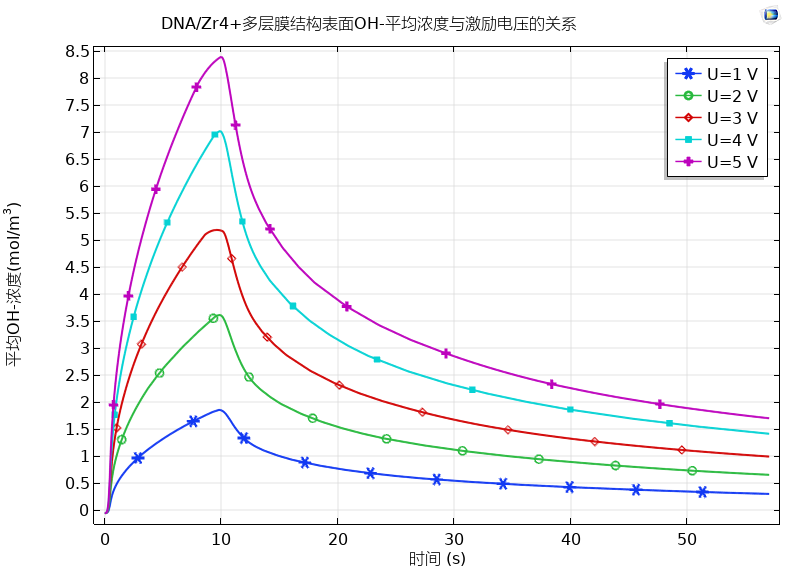
\includegraphics[width=13cm]{不同电压激励下cOH平均浓度曲线.png}
    \caption{不同电压激励下阴极表面$\ce{OH-}$浓度随时间的变化曲线}
    \label{fig:cOH_U}
\end{figure}

定义集中系数$C$为$\ce{OH-}$浓度曲线峰值的4次方除以一个信号周期内
$\ce{OH-}$浓度的4次方的积分值\footnote{
    由反应速率方程可知,水解反应的反应速率与$\ce{OH-}$浓度的4次方成正比,
    所以这里用$c_{\ce{OH-}}^4$作为参数。
}:
\begin{equation}
    C=\frac{c_{\ce{OH-},max}^4}{\int_0^T{c_{\ce{OH-}}^4}dt}
\end{equation}

集中系数$C$反映了$\ce{OH-}$浓度曲线峰值相对于整个周期内$\ce{OH-}$浓度曲线的大小。

在激励结束后滞后的$c_{\ce{OH-}}$曲线造成水解反应持续发生,对
DNA浓度观测值造成的干扰。集中系数$C$越高,
激励电压施加时发生的水解反应越占主导地位,反映了该系统的抗码间干扰能力。

由表~\ref{tab:1}可知,
随着激励电压的增加,该系统的集中系数$C$变化不大,处于缓慢的震荡减少状态。
所以我们认为激励电压的大小对码间干扰的影响不大,随着激励电压升高,码间干扰会
有轻微增加,但不影响其性能表现。

\begin{table}

    % table caption is above the table
    
    \caption{不同电压激励下集中系数$C$}
    
    \label{tab:1}       % Give a unique label
    
    % For LaTeX tables use
    \centering
    \begin{tabular}{ll}
    
    \hline\noalign{\smallskip}
    
    电压($V$) & 集中系数 \\
    
    \noalign{\smallskip}\hline\noalign{\smallskip}
    
        \quad 1&\quad 0.1800  \\
        \quad 2&\quad 0.1741  \\
        \quad 3&\quad 0.1529  \\
        \quad 4&\quad 0.1632  \\
        \quad 5&\quad 0.1518  \\
    
    \noalign{\smallskip}\hline
    
    \end{tabular}
    
\end{table}

但本文未考虑电流的热效应影响,在高电压激励下,电解产生的热量会对系统造成影响,甚至破坏DNA结构,造成信息损失,
所以系统有一个最高电压,激励电压超过了该值会对系统的稳定性产生负面的影响。

综上所述,在安全电压范围内,激励电压越高,系统的抗信道间干扰能力越强。

\subsection{激励时长的影响}

我们考虑不同持续时间的5$V$激励电压信号对电解过程的影响,在COMSOL Multiphysics中对
激励时长进行参数扫描,得到结果如图~\ref{fig:cOH_t}所示,长时间的激励可以使$\ce{OH-}$
浓度处于一个较高水平,这将增加DNA的释放量,对抗信道间干扰有利。
\begin{figure}[H]
    \centering
    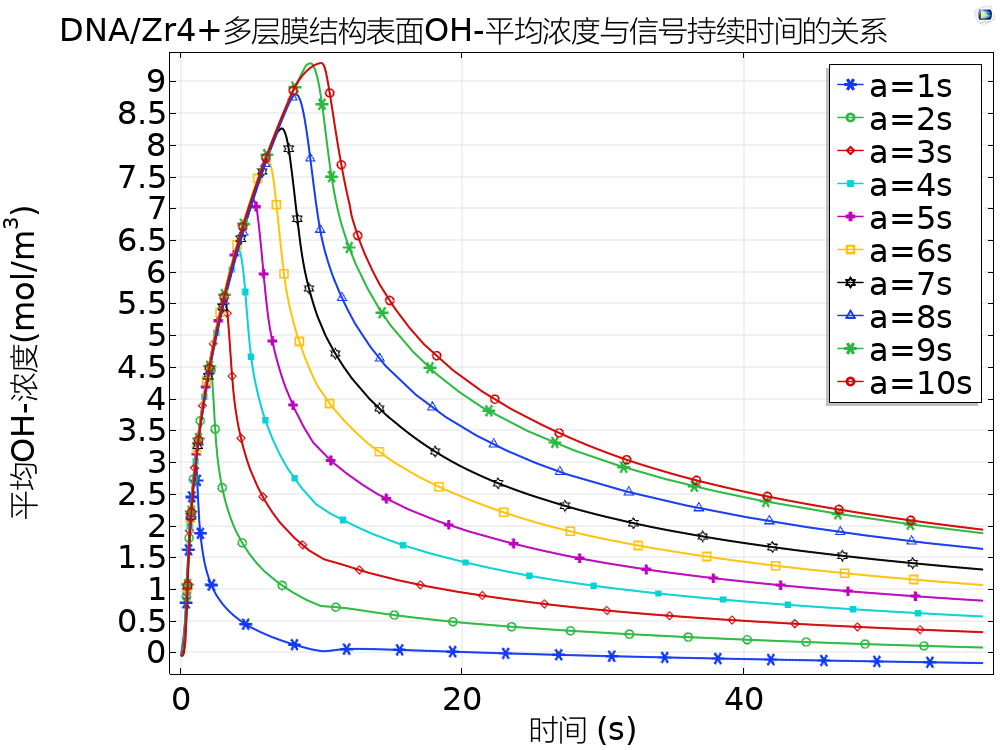
\includegraphics[width=13cm]{不同时间信号下cOH平均浓度曲线_2.png}
    \caption{不同激励时长下阴极表面$\ce{OH-}$浓度随时间的变化曲线}
    \label{fig:cOH_t}
\end{figure}

接着计算不同激励时长下的集中系数$C$,得到的结果如图~\ref{集中系数与时长}所示,
持续时间长的激励信号,其集中系数较低,这会导致其抗码间干扰能力下降,不能持续长时间
发送信号。
\begin{figure}[H]
    \centering
    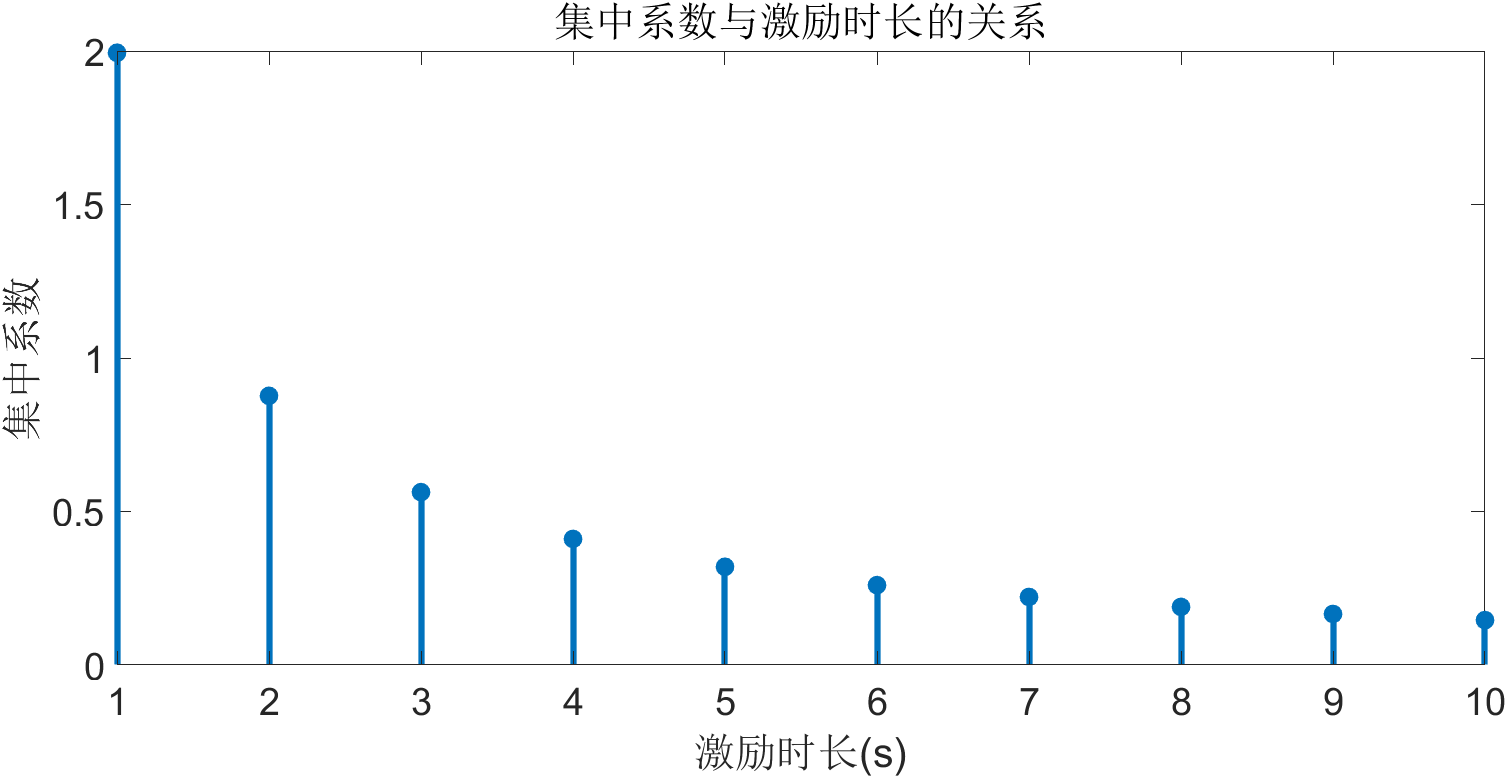
\includegraphics[width=13cm]{集中系数与时长.png}
    \caption{集中系数与激励时长的关系}
    \label{集中系数与时长}
\end{figure}

综合抗码间干扰与抗信道间干扰的能力看,激励信号应有持续时间较短、激励电压较高的特性,高电压的脉冲函数是一个理想的信号源。

\section{接收机位置对最大传输速率的关影响}
\subsection{观测点与激励信号对DNA浓度曲线的影响}

在COMSOL Multiphysics中进行电泳的仿真后,我们修改探针的位置,得到不同位置的探针的DNA浓度曲线。
激励电压我们对比原始数据的5$V$10$s$激励与5$V$1$s$的激励。

如图~\ref{不同激励探针DNA曲线}所示,
距离阴极越近的位置,DNA浓度达到峰值的时间越短,峰值强度越大。在距离
超过10$cm$之后,由于扩散速度受限,在下一次激励之前,DNA浓度不能达到峰值。所以可以得出结论
该系统通信距离越短,通信效果越好。


对比10$s$时长信号与1$s$时长信号激励下的DNA浓度曲线,可以发现在短时长信号的激励下,相同位置处,
DNA浓度峰值会更早到达,峰值相对于整条曲线也会更突出。这也佐证了上一节我们提到的,一个激励时长较短
的信号能更加有效的抑制干扰这一观点。我们也可以得出激励时长较短的信号有助于提高通信频率这一结论。
\begin{figure}[H]
    \centering
    \subcaptionbox{5$V$10$s$激励下不同位置探针的DNA浓度曲线}% 
                    [14cm]{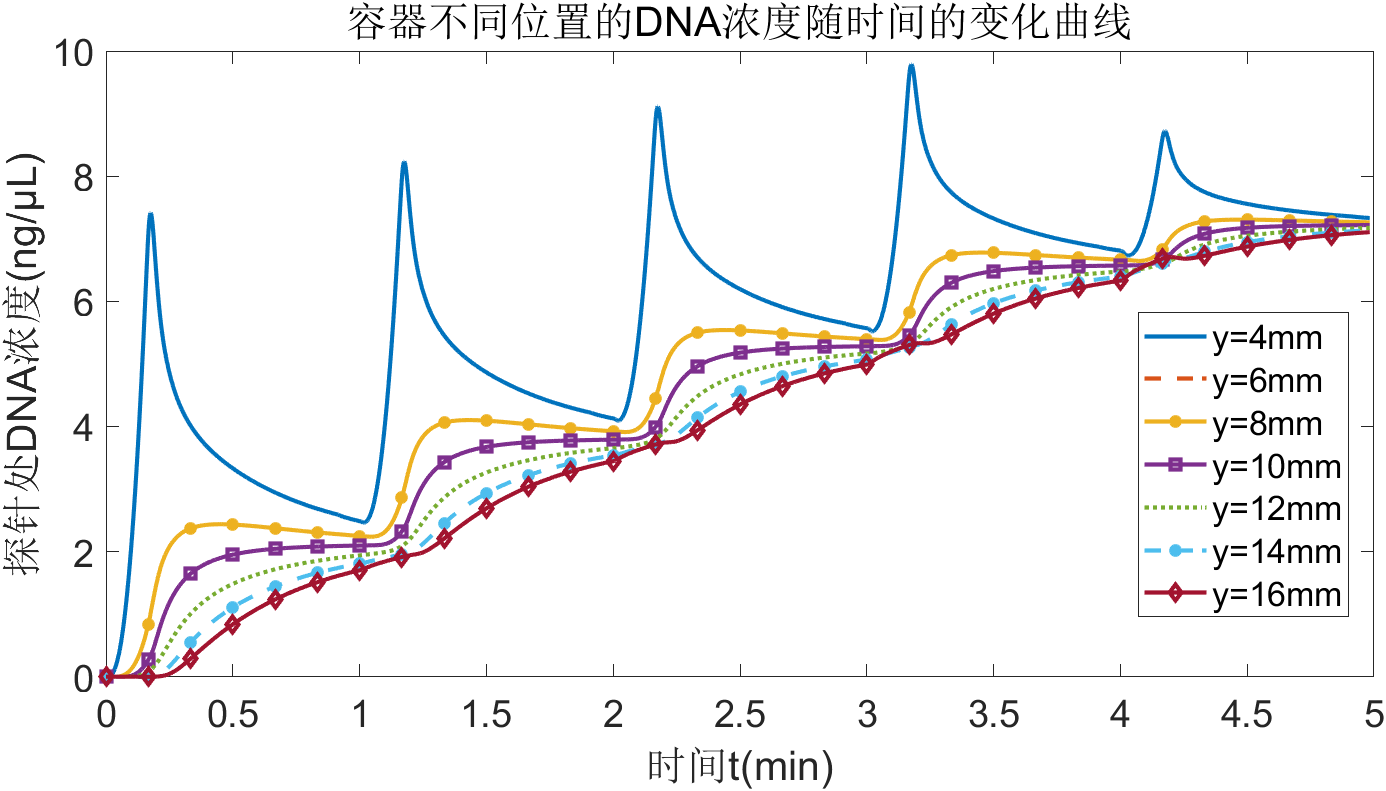
\includegraphics[width=13cm]{cDNA与t与y.png}}\\
    \subcaptionbox{5$V$1$s$激励下不同位置探针的DNA浓度曲线}% 
                    [14cm]{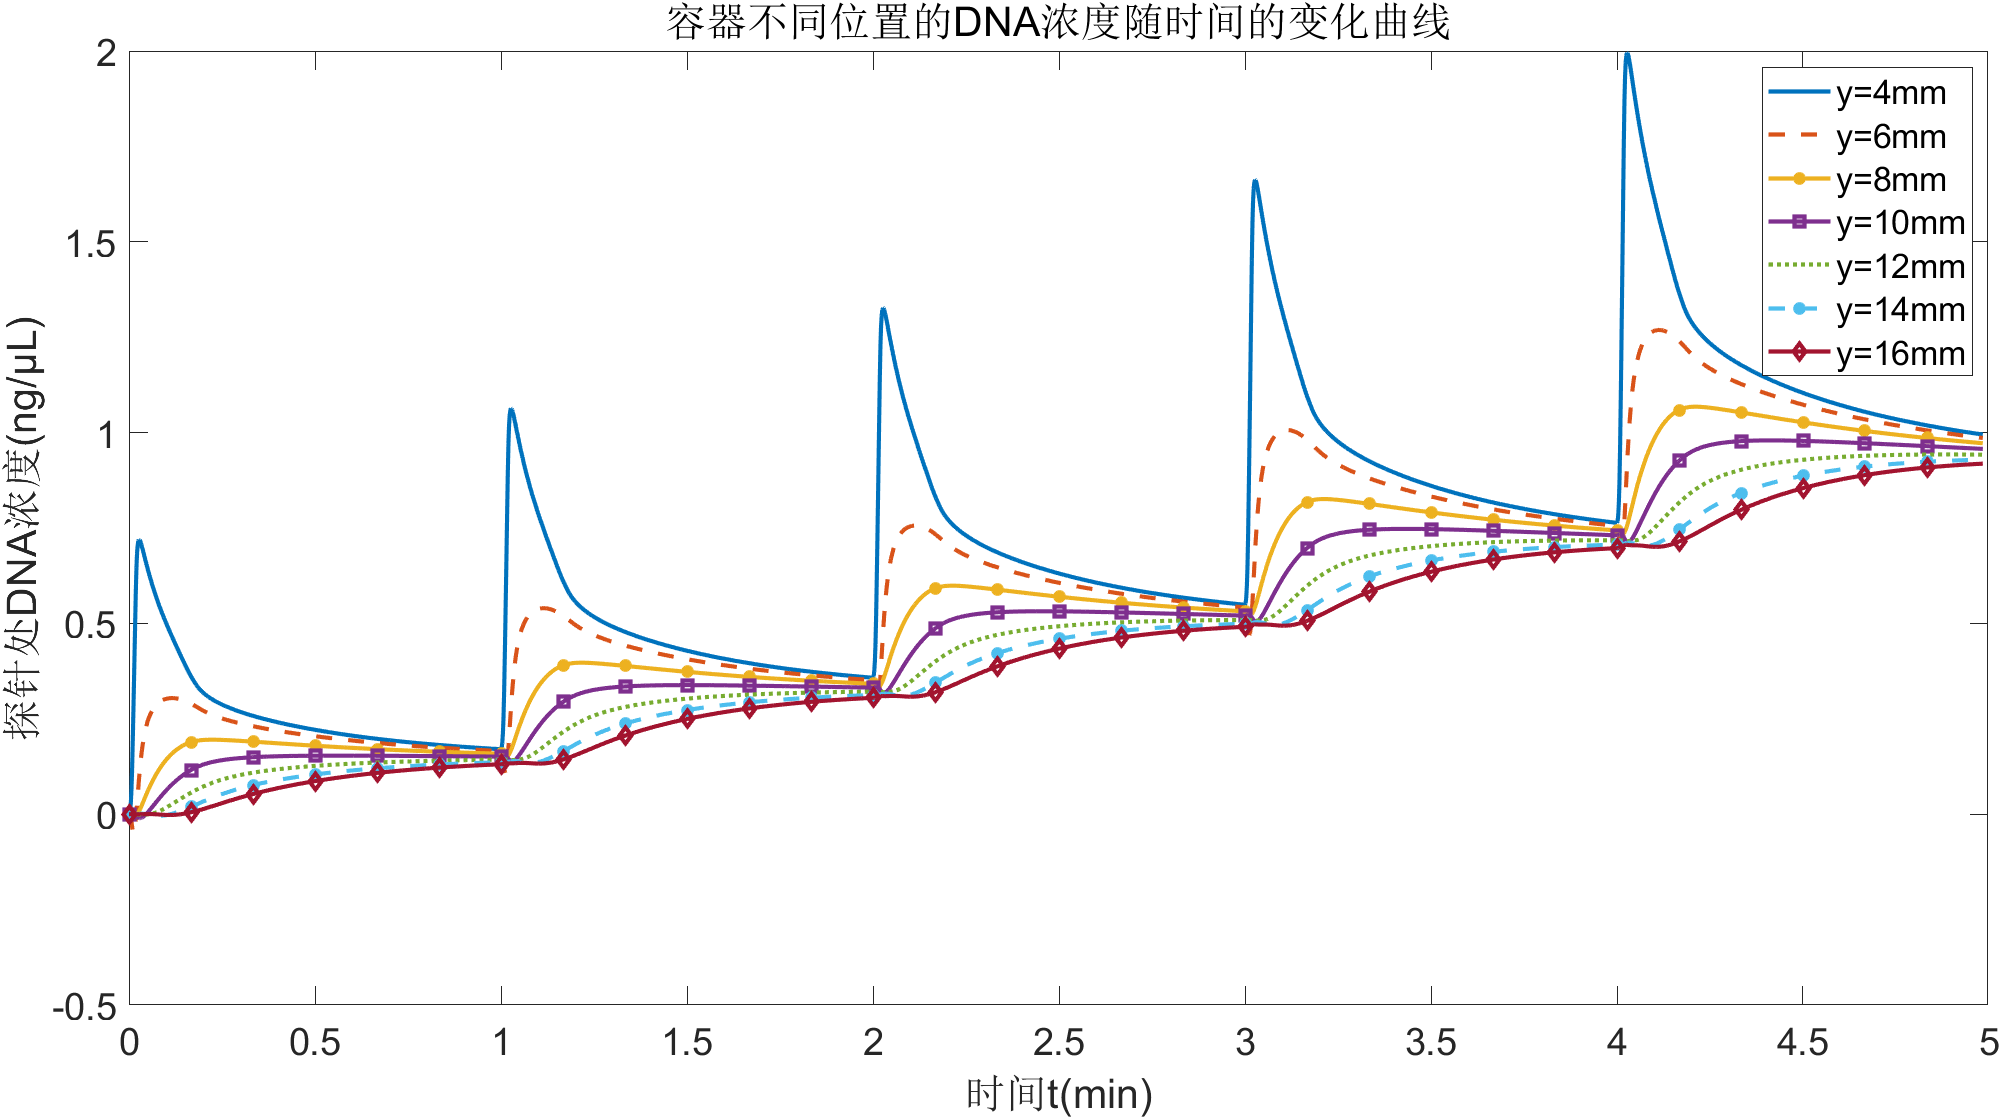
\includegraphics[width=13cm]{cDNA与t与y_1.png}}\\
    \caption{不同激励信号下不同位置探针的DNA浓度曲线}
    \label{不同激励探针DNA曲线}
\end{figure}

\subsection{不同观测点的最大通信频率}

我们定义DNA浓度在单次激励中的的上升时间$T_s$为其达到该信号周期
内浓度最大值$c_{max}$的$\frac{1}{\sqrt{2}}$时,
所用的时间。图~\ref{rising time}显示了在激励电压为5$V$,激励时长为1$s$的信号作用下,
距离阴极不同位置的观测点,DNA浓度的上升时间及其倒数。

\begin{figure}[H]
    \centering
    \subcaptionbox{离阴极不同距离的观测点处DNA浓度的上升时间}% 
                    [14cm]{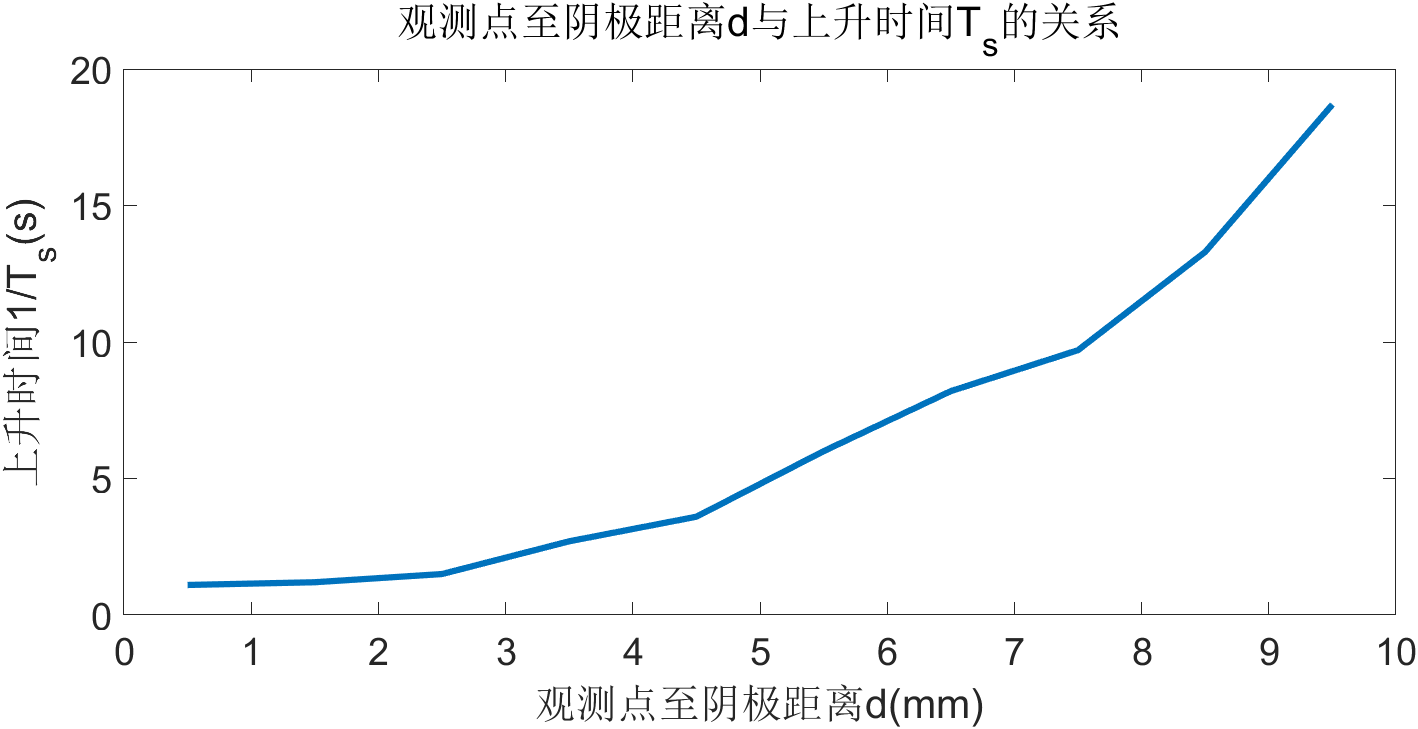
\includegraphics[width=13cm]{raising time.png}}\\
    \subcaptionbox{离阴极不同距离的观测点处DNA浓度的上升时间的倒数}% 
                    [14cm]{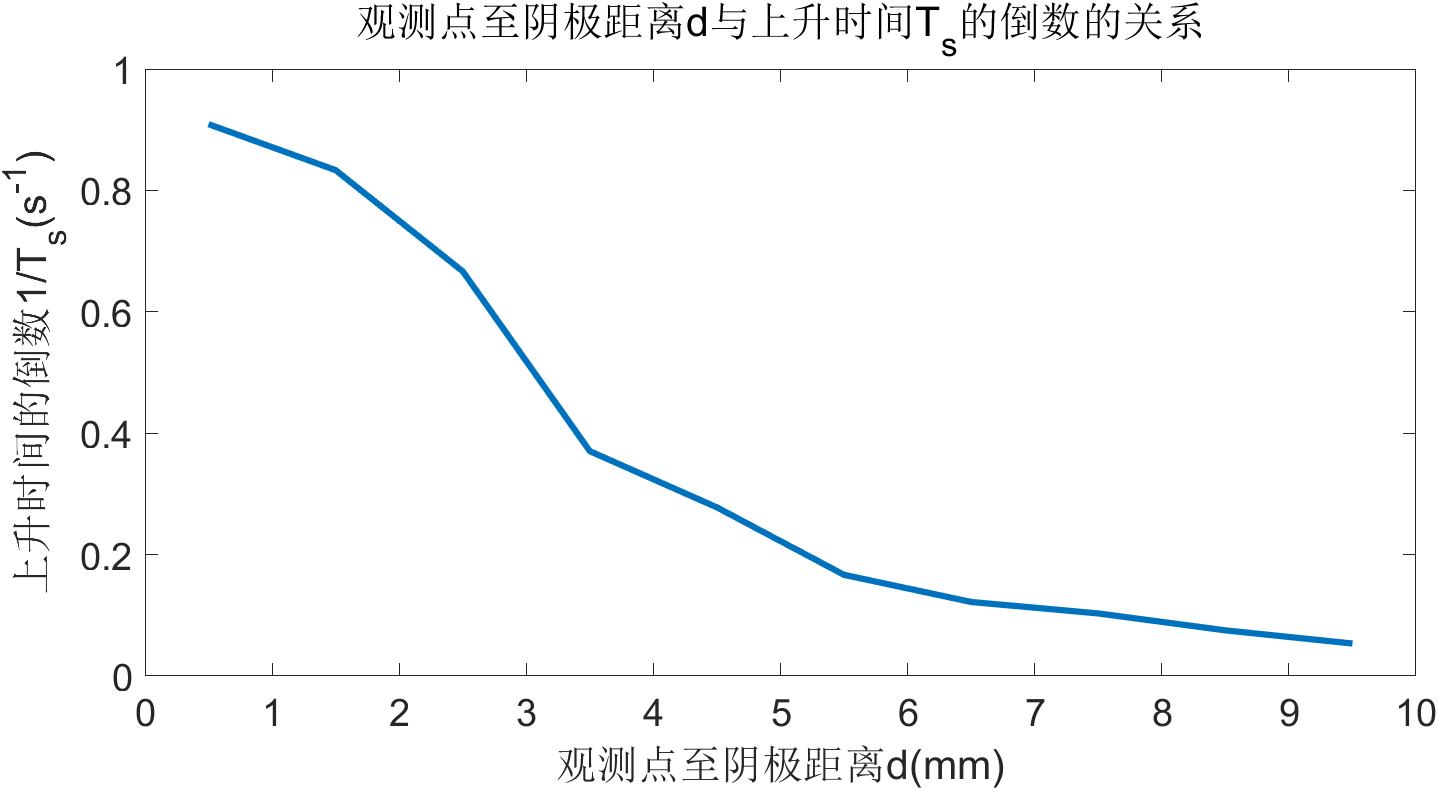
\includegraphics[width=13cm]{raising_time_frequency.png}}\\
    \caption{离阴极不同距离的观测点处DNA浓度的上升时间及其倒数}
    \label{rising time}
\end{figure}

我们可以将达到浓度最大值$c_{max}$的$\frac{1}{\sqrt{2}}$时的时刻作为采样点,这时
最大通信频率为上升时间的倒数。图~\ref{rising time}的数据显示,在距离阴极0.5mm的地方,
我们可以达到0.909Hz的最大通信频率;在距离阴极4.5mm处,我们可以达到0.2778Hz的最大通信频率,
而在距离阴极9.5mm处,最大通信频率只有0.05348Hz。

数据说明了,基于自由扩散的通信系统,不适合远距离通信。接收机放置在距发送机5$mm$这一范围内时,
能达到一个较快的通信速度,而且抗干扰能力强。在超过7$mm$这一范围后,通讯的间隔必须增加到数十秒,
以抑制码间干扰,而且其抗信道间干扰能力也会下降。

\section{系统阈值}
\subsection{基于水解反应的$c_{\ce{OH-}}$阈值}
由$\ce{Zr^4+}$的水解方程~\ref{Zr4+水解}可以得知,
$\ce{Zr^4+}$参与水解的条件应该为:
\begin{equation}
    \frac{c_{\ce{H+}}^4}{c_{\ce{Zr^4+}}  }<K°=10^{1.9}
\end{equation}

由水溶液中存在水的电离,将$\ce{H+}$与$\ce{OH-}$的浓度相联系,可以将上述式子变形为:
\begin{equation}
    \frac{k_w^4}{c_{\ce{Zr^4+}} c_{\ce{OH-}}^4 }<K°=10^{1.9}
\end{equation}

即当$c_{\ce{OH-}}$满足如下条件时,水解反应才会开始:
\begin{equation}
    c_{\ce{OH-}}>\frac{k_w}{(c_{\ce{Zr^4+}}K°)^{1/4}}
\end{equation}

其中$K°=10^{1.9}$,$K_w=10^{-14}$。考虑$\ce{Zr^4+}$在LbL结构中的离子间间距为3~4$nm$
\cite{\cite{Shervedani2011Electrochemical}},由此计算其在阴极表面的活度
\footnote{又称有效浓度,有效摩尔分数}:
\begin{equation}
    c_{\ce{Zr^4+}}=(\frac{1dm}{3.5nm})^3\cdot \frac{1}{N_A} mM
    =0.0387mM
\end{equation}

其中$N_A$为阿伏伽德罗常量,取$6.022\times 10^{23}$。计算得到$c_{\ce{OH-}}$的阈值为
$7.55\times 10^{-15}mM$,该水解反应启动的浓度阈值非常小,可以认为在$\ce{OH-}$存在时,反应
都会发生,由于反应速度与$c_{\ce{OH-}}$的4次方成正比,所以低浓度时,反应速度极慢,在所观测的
时间尺度下,可以认为不施加激励电压时反应不发生。
\subsection{基于电化学反应的电压阈值}

在式~\ref{equation:Butler_Volmer}中我们提到了,在电化学反应中,施加的电压必须超过平衡电压,
即过电位应大于0时,反应才会正向发生。引用\parencite{C9RP00218A}一文的介绍,对于本文中的溶液环境,
理论上电化学反应的开启电压为1.229$V$,考虑式~\ref{equation:cathode_reaction}中水直接参与
电极反应所需要的能量,该电化学反应的电压阈值应为2.17$V$,但是在实际条件下,
由于电极阻抗、溶液电导率等因素的影响,可能需要更大的电压来启动此反应\footnote{
    https://chemed.chem.purdue.edu/genchem/topicreview/bp/ch20/faraday.php\#aq
},如工业上电解食盐水的实际电压在3.5~4.0$V$。

\subsubsection{DNA/$\ce{Zr^4+}$单层的释放次数}
在激励电压为5$V$激励时长为1$s$的信号作用下,$\ce{Zr^4+}$的消耗曲线如图~\ref{5_1_Zr曲线}所示。由于
$\ce{Zr^4+}$的消耗,DNA也被释放进入溶液中,LbL结构分解。我们可以得到在该激励信号的作业下,每次激励
消耗的$\ce{Zr^4+}$/DNA单层会被消耗16\%。所以理论上,在高电压、短时长激励信号的作用下,
每一层$\ce{Zr^4+}$/DNA单层最多可以释放6次。

\begin{figure}[H]
    \centering
    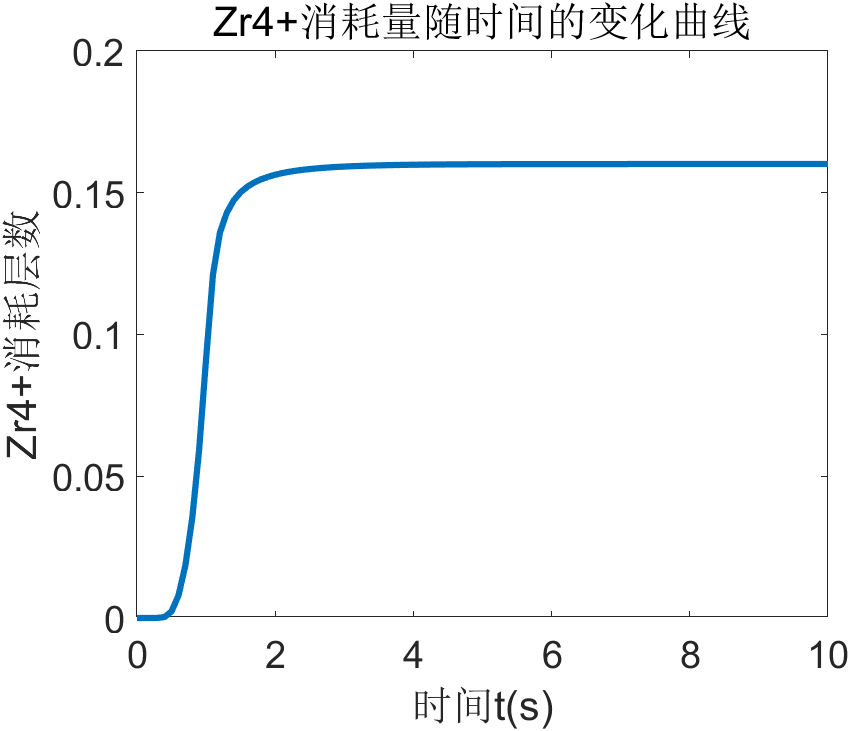
\includegraphics[width=8cm]{Zr阈值.png}
    \caption{5$V$1$s$激励下$\ce{Zr^4+}$消耗曲线}
    \label{5_1_Zr曲线}
\end{figure}



